\documentclass[3p,review,12pt]{elsarticle}
\usepackage{lineno,hyperref,notoccite,etoolbox}
\modulolinenumbers[5]
\makeatletter
\def\ps@pprintTitle{%
	\let\@oddhead\@empty
	\let\@evenhead\@empty
	\def\@oddfoot{\centerline{\thepage}}%
	\let\@evenfoot\@oddfoot}
\makeatother
\usepackage{setspace}
\singlespacing
\usepackage{mathptmx}
\usepackage{float,wrapfig}
\newcommand{\vs}{\vspace{2mm}}
\begin{document}

\begin{frontmatter}
	\title{Computational Methods for Amorphous Semiconductor Devices}
	
	\author[boise]{Ember L. Sikorski}
	
	
	\address[boise]{Boise State University}
	
	\begin{abstract}

We examine four computational methods applicable to amorphous materials: Density Functional Theory (DFT), \textit{Ab initio} Molecular Dynamics (AIMD), Molecular Dynamics (MD), and Monte Carlo (MC). Each method has been used to better understand amorphous materials including amorphous perovskites, amorphous alumina, amorphous Si, and amorphous phase change materials. The lower length scale methods can calculate electronic properties, such as density of states, and structural properties of a small unit cell. The higher length scales can treat hundreds and thousands of atoms and show evolution with time. Selection of a computional method requires a clear definition of the system of interest and properties of interest. Computational methods exhibit a negative correlation between accuracy and speed. Selection of energy functionals and pair-potentials requires a literature review to verify such a method is appropriate for the desired system. 

	\end{abstract}
	
	
\end{frontmatter}
\tableofcontents
\section{Introduction}
\begin{figure}[h]
	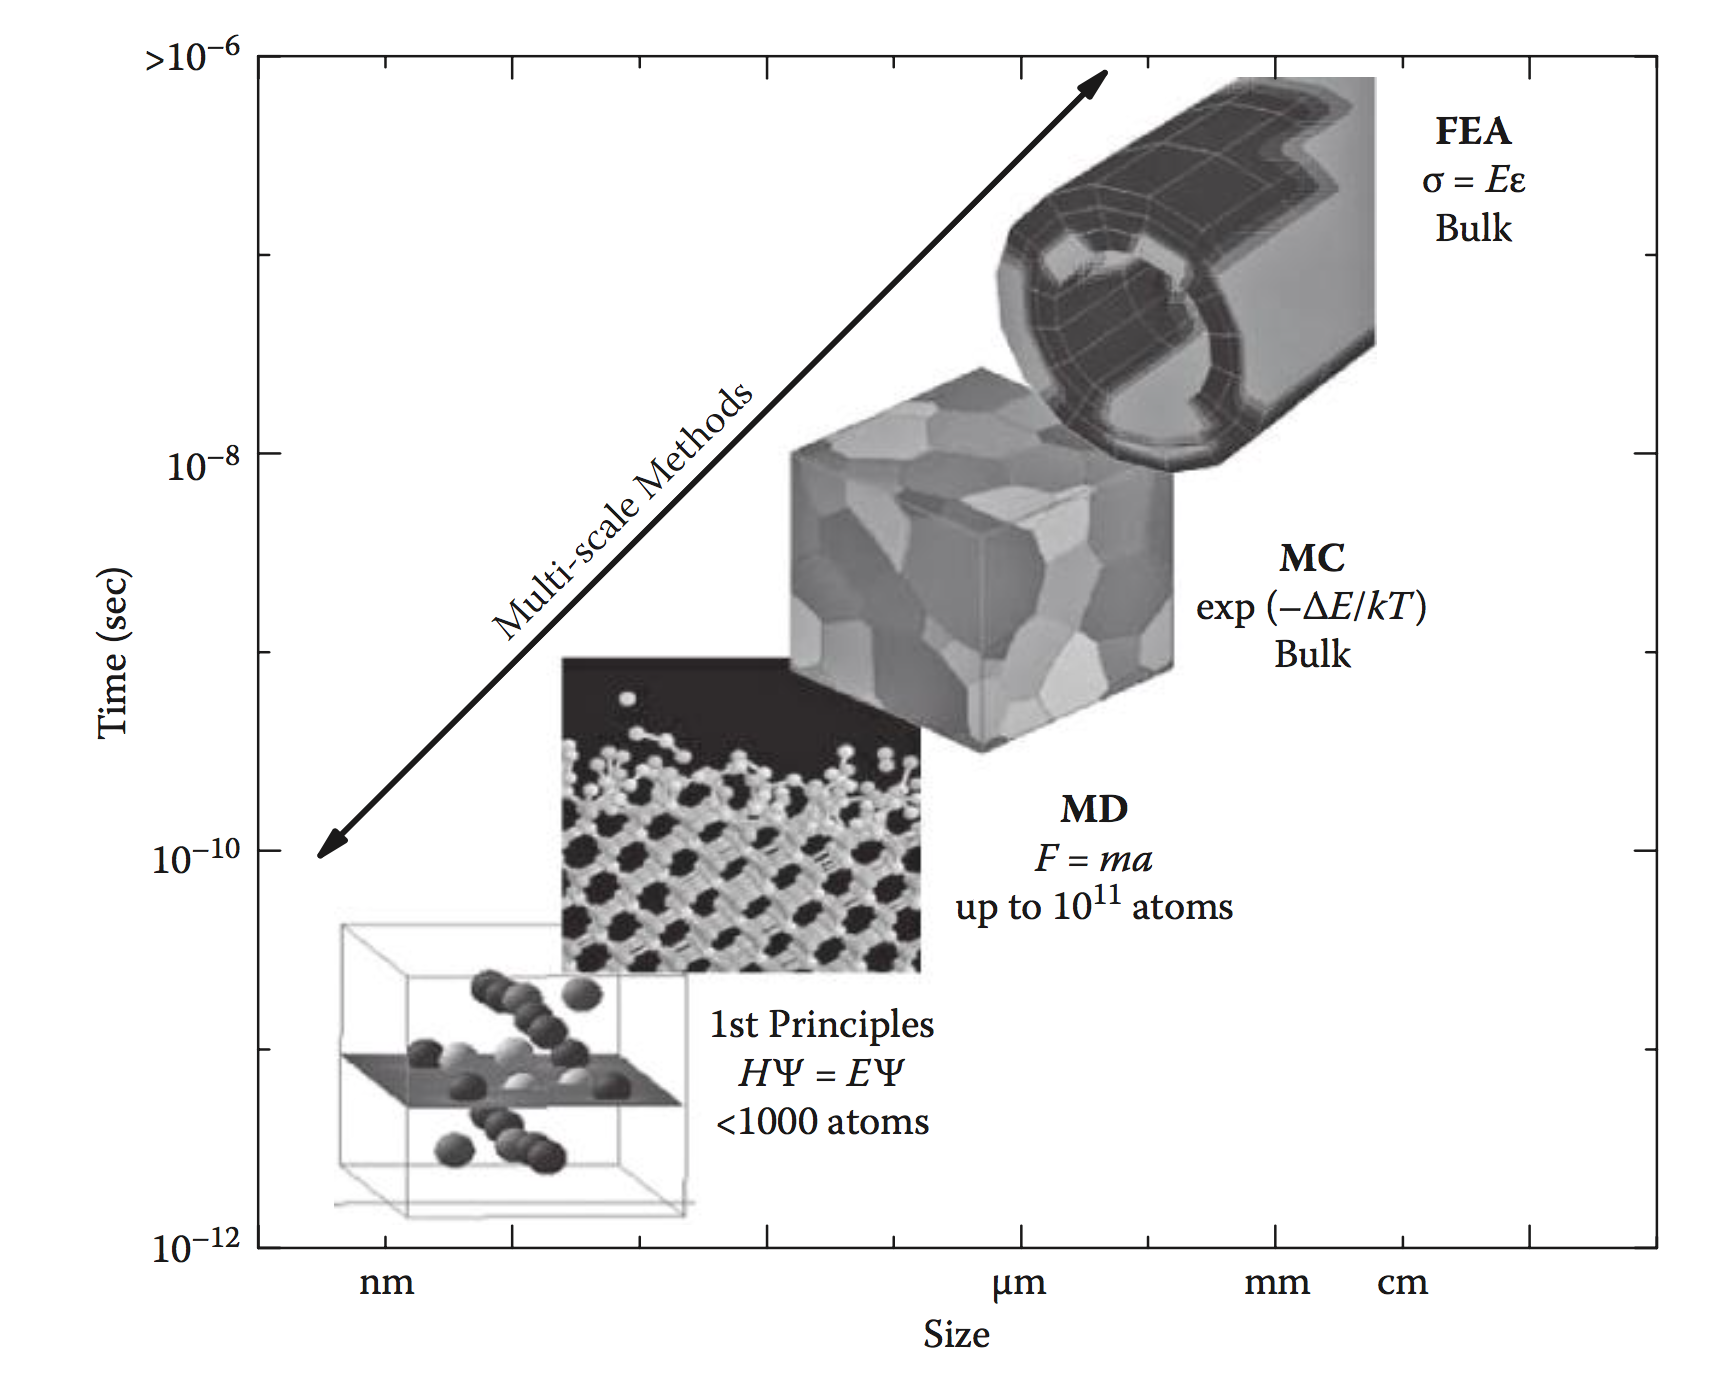
\includegraphics[width=0.5\textwidth]{overview}
	\centering
	\caption{Overview of computational methods with respect to time and size capabilities. \cite{Lee2012}}
\end{figure}
Computational modeling can greatly assist experimental studies of materials. When starting from experiment, modeling can help determine the mechanism of a process or the structure of a material. When starting from computation, modeling can screen an array of materials to predict which will yield the best properties.
\par
Computational modeling spans length scales from the order of meters, that we experience, to the order of \aa ngstr\"oms, that atoms experience. Due to this vast range of length scales, no one method can address all properties. Following, computational methods are broken down into four main categories (\textbf{Fig. 1}): First principles or \textit{ab initio}, molecular dynamics (MD), mesoscale methods such as Monte Carlo (MC), and continuum methods such as finite element analysis (FEA)\cite{Lee2012}. This review focuses on the lower three: first principles, MD, and MC, which can be used to find the structure of amorphous materials. Density of states is an inherently electronic calculation, and as such can only be calculated from first principles. We will additionally study \textit{Ab initio} Molecular Dynamics, a combination of the lower two length scales, which we will see is particularly useful for amorphous materials. For each method, we discuss the theory and an example of its application for amorphous materials. Our examples will include determining the structural and electronic origin of photoluminescence in amorphous perovskites, determining the basic units of amorphous alumina, finding the structure of a-Si using diffraction results, and probing the mechanism of aging in phase change materials. Lastly, we will discuss the benefits and drawbacks of each method, how to select a method,  and what considerations must be taken into  account in a computational study.




\section{First Principles}
\subsection{Formulation of Density Functional Theory}
First principles, or \emph{ab initio}, modeling is derived solely from quantum mechanics and considers the nuclei and atoms of a system. The term "first principles" refers to the models ability to solve for electronic and structural properties knowing only the constituent atomic species or, rather, no experimental input. The method is based on the Schr\"odinger's equation. However, this equation can only be analytically solved for hydrogen. To extend its applicability, several assumptions and approximations must be made to yield density functional theory (DFT).
\par 
In short, DFT does not consider gravity, relativity, or excited states \cite{Lee2012}. The nuclei and electrons are considered separately, known as the Born-Oppenheimer approximation, as nuclei are 10,000 times more massive than electrons, in the case of semiconductors, and the electrons will instantaneously move with them.  These simplifications yield the following Hamiltonian:

\begin{equation}
\hat{H}=-\frac{1}{2}\sum_{i}^{n}\nabla_{i}^{2}-\sum_{I}^{N}\sum_{i}^{n}\frac{Z_{I}}{|\vec{r}_{Ii}|}+\sum_{i\neq j}^{n}\frac{1}{|\vec{r}_{ij}|} \qquad 
\end{equation}
where $N$ is the number of nuclei, $n$ is the number of electrons, $Z_{I}$ is the charge of the nuclei, $\nabla^{2}$ is the Laplacian operator, and $\vec{r}$ is the position. The first term is the kinetic energy, the second is the potential between electrons and nuclei, and the third is the potential between electrons. Energy is calculated by taking the expectation value of the Hamiltonian:
\begin{equation}
	E = \sum_{i,j} \int \Psi_{i}^{*} (\vec{r}) \Bigg(-\frac{1}{2}\sum_{i}^{n}\nabla_{i}^{2}-\sum_{I}^{N}\sum_{i}^{n}\frac{Z_{I}}{|\vec{r}_{Ii}|}+\sum_{i\neq j}^{n}\frac{1}{|\vec{r}_{ij}|}\Bigg)\Psi_{i}(\vec{r})d\vec{r}
\end{equation}
 The Hartree-Fock method introduces the Slater determinant to include antisymmetry. The Kohn-Sham approach is applied to turn the \emph{n}-electron system into a fictitious system of one-electrons. Solving the Kohn-Sham Hamiltonian yield the Kohn-Sham orbitals $\phi_{i}(\vec{r})$:
 
 \begin{equation}
 \bigg[-\frac{1}{2}\nabla^{2}+U_{eff}(\vec{r})\bigg]\phi_{i}(\vec{r}) = \epsilon_{i}\phi_{i}(\vec{r}) \Rightarrow \hat{H_{KS}}\phi_{i} = \epsilon_{i}\phi_{i}(\vec{r}) \qquad ,
 \end{equation}
where $\epsilon_{i}$ are the Kohn-Sham eigenvalues. The electron density is then found by summing over the squares of the non-interacting Kohn Sham orbitals:

\begin{equation}
\rho (r) = \sum_{i}|\phi _{i}(r)|^{2} \qquad.
\end{equation}
The third term of the Hamiltonian, the potential energy between electrons, is split into Hartree energy and exchange-correlation energy. The Hartree energy is  the potential felt on each electron by a homogeneous electron gas of all the other electrons. Exchange energy describes the interaction of same spin electrons and correlation energy describes the interaction of different spin electrons. Though exchange-correlation energy is small in magnitude compared to the other energetic terms, it is directly linked to the accuracy of the method, as shown in \textbf{Fig. 2}. 


\begin{figure}[h]
	\centering
	\begin{minipage}[b]{0.45\textwidth}
		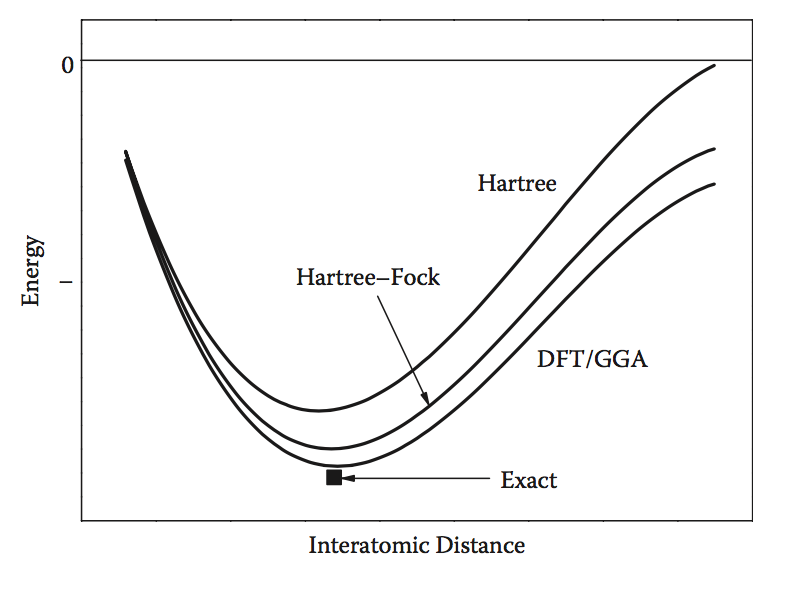
\includegraphics[width=\textwidth]{lee1}
	\end{minipage}
	\hfill
	\begin{minipage}[b]{0.45\textwidth}
		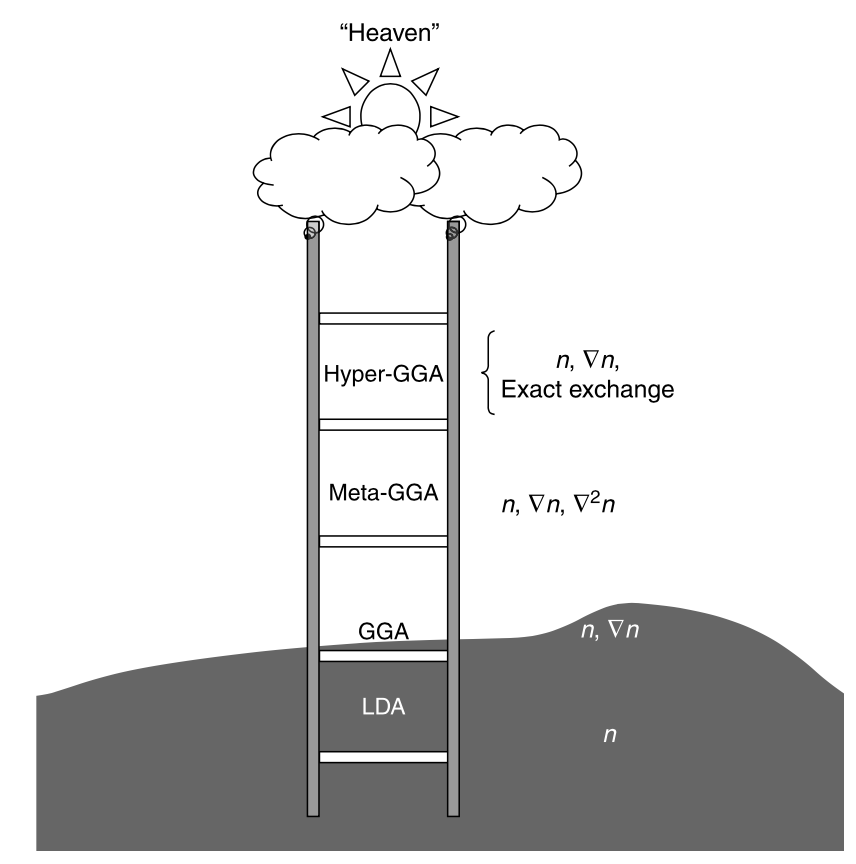
\includegraphics[width=0.8\textwidth]{sholl1}
		\centering
	\end{minipage}
	\caption{Energy schematic \cite{Lee2012} (left) and Jacob's ladder depiction \cite{Sholl2009} of various functionals.}
\end{figure}

Three main categories of exchange-correlation functionals are the Local Density Approximation (LDA), Generalized Gradient Approximation (GGA), and hybrid functionals. Hybrid functionals, also referred to as meta-GGA , combine Hartree Fock with DFT functionals. Perdew, of PBE - a revision to GGA \cite{Perdew1996}, introduced the analogy of the Jacob's ladder in \textbf{Fig. 2}. Going up the ladder represents increasing accuracy when compared with experiment, but it is done at computational cost. Any functional at the third rung or above is at least ten times as expensive as GGA \cite{Lee2012}. Though the Jacob's ladder is presented as a linear progression between functionals, this is a large simplification and the accuracy of a functional is often system-dependent. Another important consideration when selecting a functional is whether it is nonempirical - based on constraints of the Kohn-Sham functional - or empirical - parameterized by experiment \cite{Sholl2009}. The B3LYP functional, for example, is an empirical potential fitted to atomization energies, ionization potentials, and other experimental values \cite{Lee2012}. It excels in describing molecular systems, van der Waals interactions, and rapidly fluctuating electron densities. However, this method is not always well suited for metals and semiconductors \cite{Paier2007}.
\par 

DFT runs using an iterative self-consistent framework shown in\textbf{ Fig. 3}. First, an electron density is created using the superposition of the pseudopotentials (mathematically simplified functions resulting from freezing core electrons with the nucleus) of each atom. Second, calculate the terms of the Kohn-Sham Hamiltonian and use the electron density to solve the exchange-correlation functional.  Third, solve the Kohn-Sham equations through direct diagonalization to obtain the Kohn-Sham orbitals. Fourth, use the new orbitals to solve for the electron density. Repeat this process until the difference in energy between calculations reaches a predetermined stopping criteria. Once the energy converges, update the nuclei positions and repeat the iterative process. The method continues until energy differences between subsequent nuclei positions reaches the stopping criteria. 

\begin{figure}[H]
	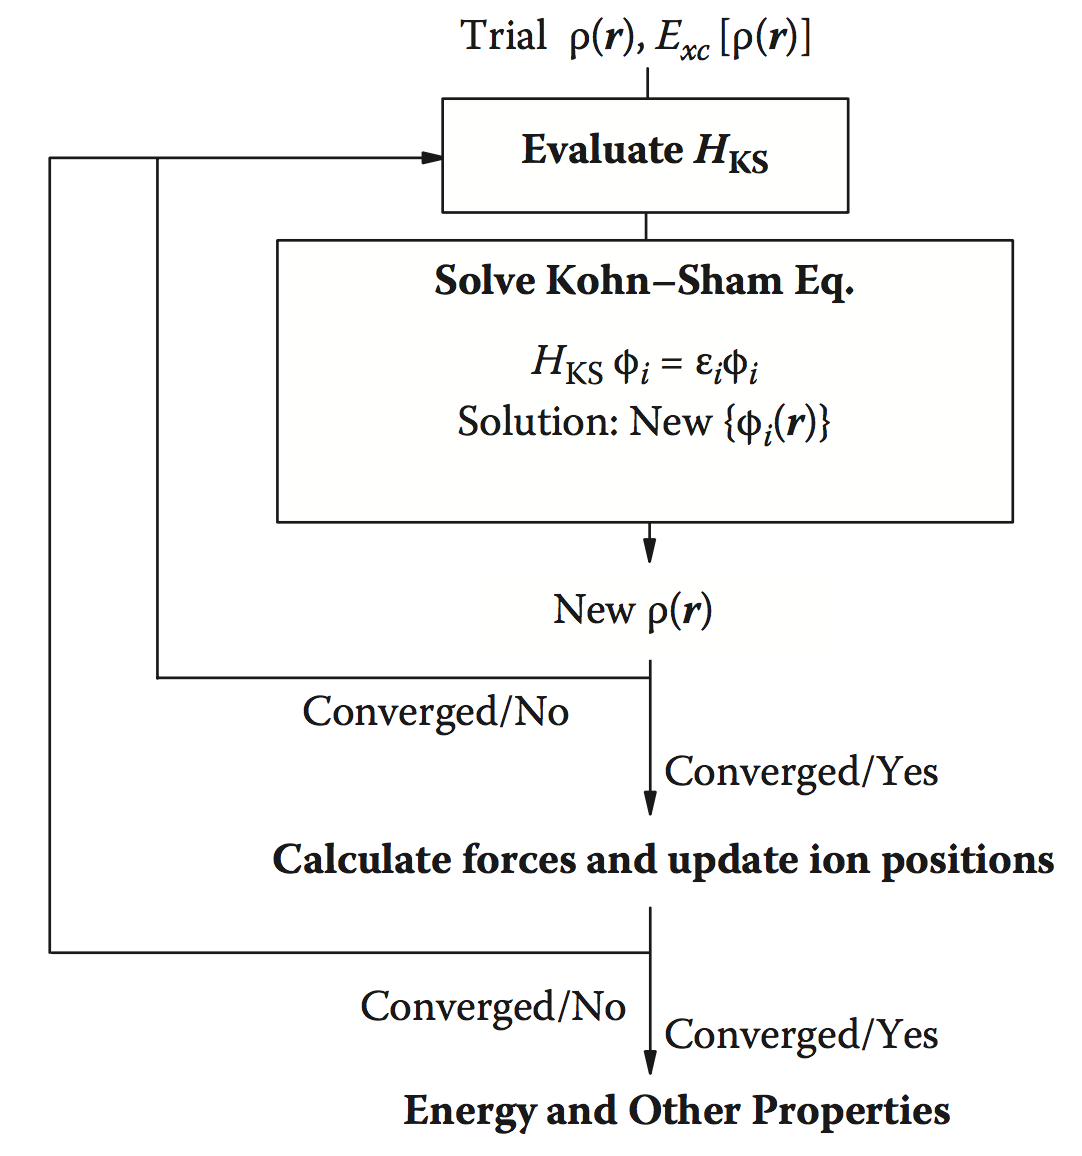
\includegraphics[width=0.6\textwidth]{scf}
	\centering
	\caption{Self-consistent framework (SFC) loop used in DFT \cite{Lee2012}.} 
\end{figure}

Once the system converges, the output wave functions and electron densities can be used to calculate electronic properties such as the Density of States (DOS). The density of states is found by integrating the electron density in reciprocal space \cite{Sholl2009}. This can further be broken down into the density of states on each atom referred to as the Local Density of States (LDOS) and in each orbital referred to as the Projected Density of States (PDOS).


\subsection{Photoluminescence in amorphous perovskites}
\begin{figure}[h]
	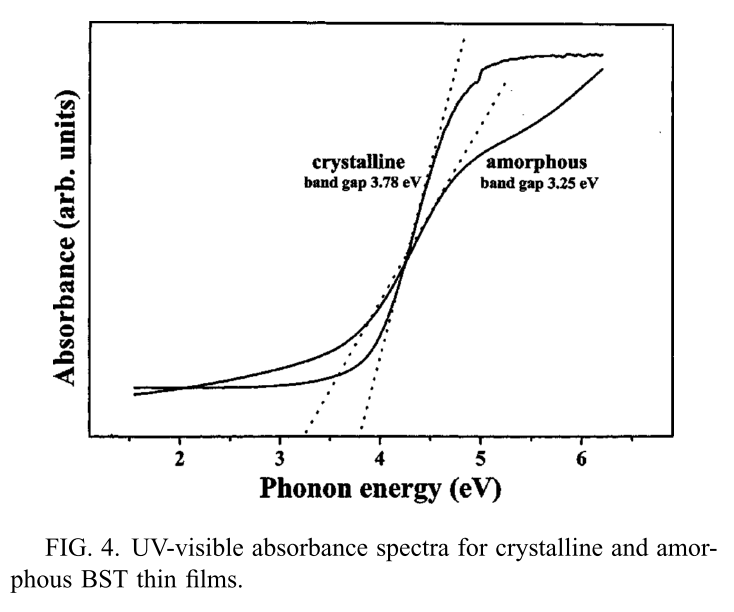
\includegraphics[width=0.6\textwidth]{longo3}
	\centering
	\caption{UV-visible absorbance spectra for crystalline and amorphous Ba$_{0.5}$Sr$_{0.5}$TiO$_{3}$ films from Longo et al. \cite{Longo2004}} 
\end{figure}


Longo et al. \cite{Longo2004} used DFT to determine the origin of photoluminescence in their amorphous titanates. They chose  crystalline and amorphous Ba$_{0.5}$Sr$_{0.5}$TiO$_{3}$ (BST) for computational analysis using the B3LYP functional. From x-ray absorption near edge spectra (XANES), they determined the amorphous titanates contained both fivefold and sixfold oxygen-titanium coordination. In order to create this coordination, they shifted the Ti atom by 0.5 $\AA$, as shown in \textbf{Fig. 6}. From the band gap in \textbf{Fig. 5}, the indirect bandgap in crystalline BST is equal to 3.78 eV, in agreement with the optical bandgap found in experiment (\textbf{Fig. 4}). For amorphous BST, this indirect bandgap decreases to 3.06 eV. The LDOS in \textbf{Fig. 5} show the valence band is made up of O states while the conduction band is made of Ti states. The authors note covalent bonding occurs between Ti and O, through the overlap of Ti 3d states and O 2p states. The nature of the bonding is further realized in \textbf{Fig. 6(a)}. A  valley exists in the surface plot between Ba and Sr, indicating ionic bonding. Conversely, the charge density between Ti and O is higher and can additionally be seen in the contour map as exhibiting regions of the same charge. These characteristics point to covalent bonding.\textbf{ Fig. 6(b)} emphasizes the distinction between the Ti-O bonds in crystalline an amorphous BST: the covalent bonds are weaker in amorphous BST as the contour map shows reduced regions of the same charge density. These results suggest that the change in the Urbach tail of the absorption spectra is due to the disorder in the amorphous structure which leads to localized states in the O 2p orbitals.

\par

Though the band gap results of Longo et al. agree well with their experimental data, the structure they modeled is not entirely amorphous. Due to their small unit cell of 1 $\times$ 1 $\times$ 2, this creates a periodic structure in which half of the Ti have distorted local bonding. If there were greater distribution of bond lengths and types, it is likely further details in the photoluminescence mechanism could be unearthed.
\par

Additionally, the B3LYP is a partially empirical functional \cite{Paier2007}. Due to the fixed nature of empirical potentials, this method may struggle in accurately representing the system if the system exhibits any anisotropy \cite{Hohl1991}. Paier et al. \cite{Paier2007} have shown that B3LYP performs poorly for metals and small gap semiconductors, which would be better described with nonempirical hybrid functionals such as PBE0 and HSE03. At the high computational cost of a hybrid functional, a nonempirical functional may be better suited for such a study.

\begin{figure}[H]
	\centering
	\begin{minipage}[b]{0.45\textwidth}
		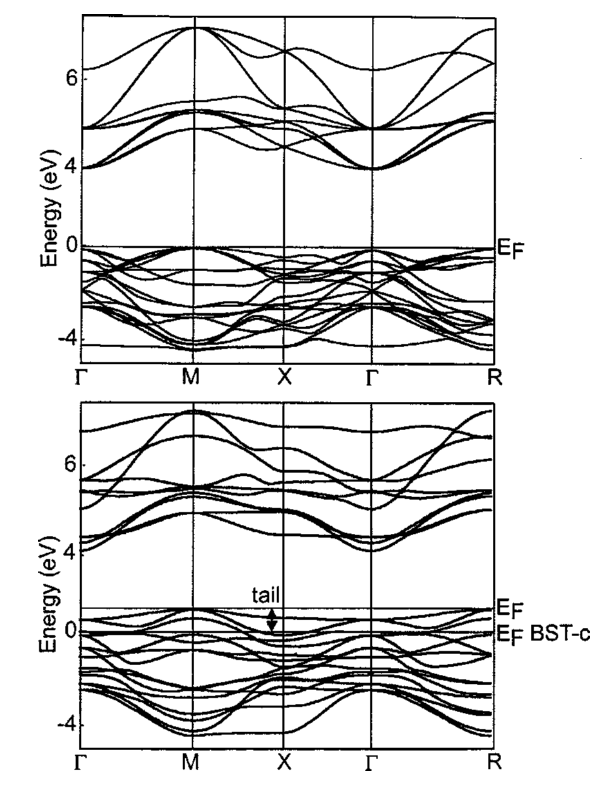
\includegraphics[width=\textwidth]{longo1}
	\end{minipage}
	\hfill
	\begin{minipage}[b]{0.45\textwidth}
		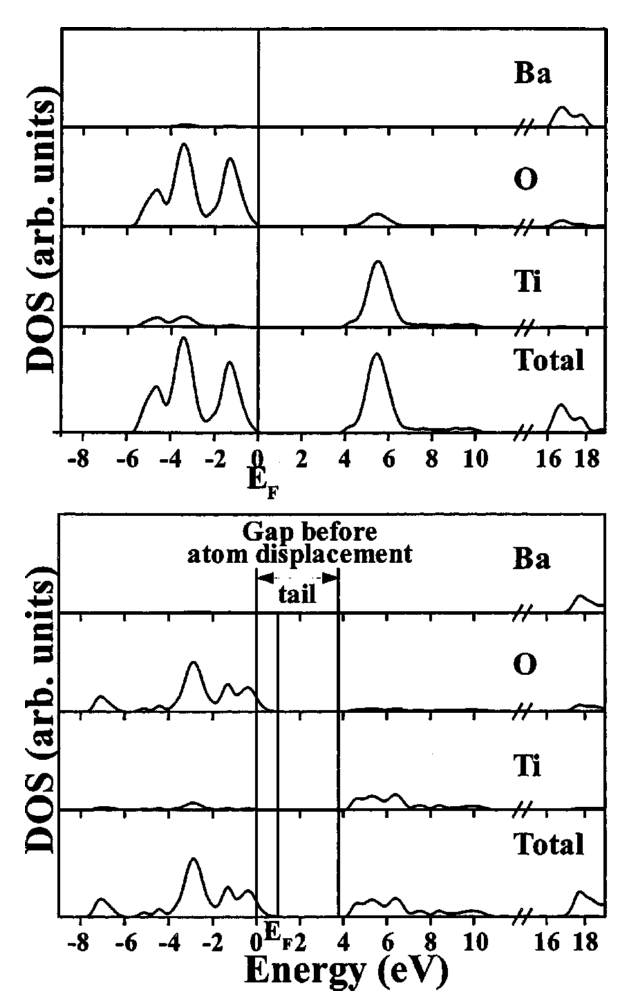
\includegraphics[width=0.82\textwidth]{longo2}
		\centering
	\end{minipage}
	\caption{Calculated band structure (left) and density of states (right) from Longo et al. \cite{Longo2004} for crystalline (top) and amorphous (bottom) Ba$_{0.5}$Sr$_{0.5}$TiO$_{3}$.}
\end{figure}
\begin{figure}[H]
	\centering
	\begin{minipage}[b]{0.45\textwidth}
		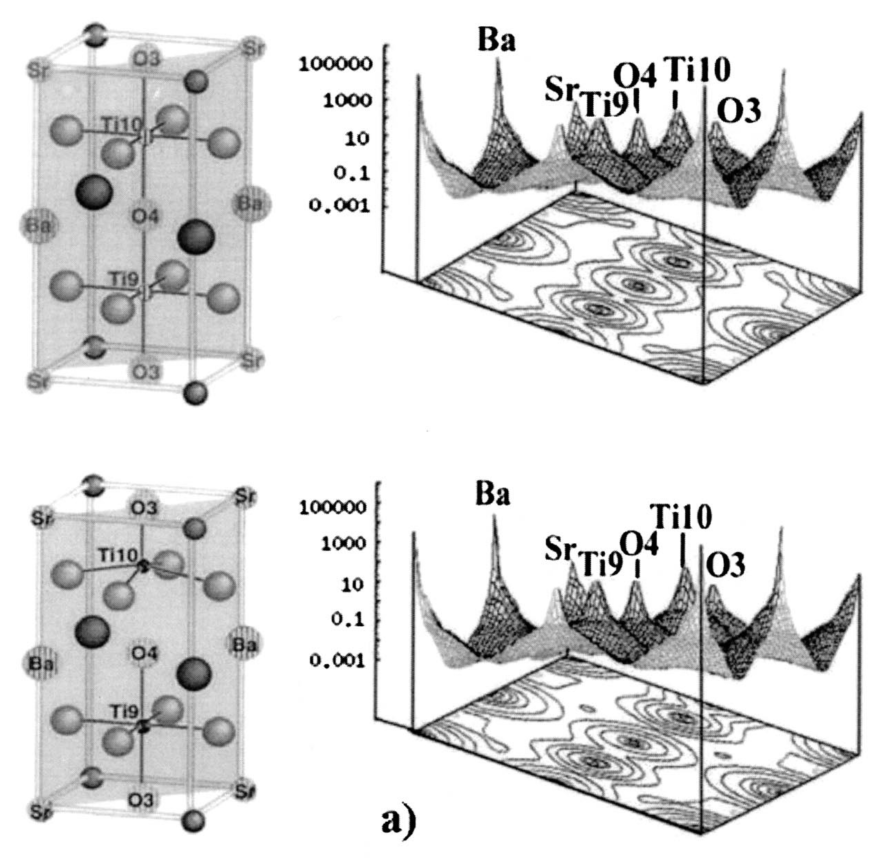
\includegraphics[width=\textwidth]{longoA}
	\end{minipage}
	\hfill
	\begin{minipage}[b]{0.45\textwidth}
		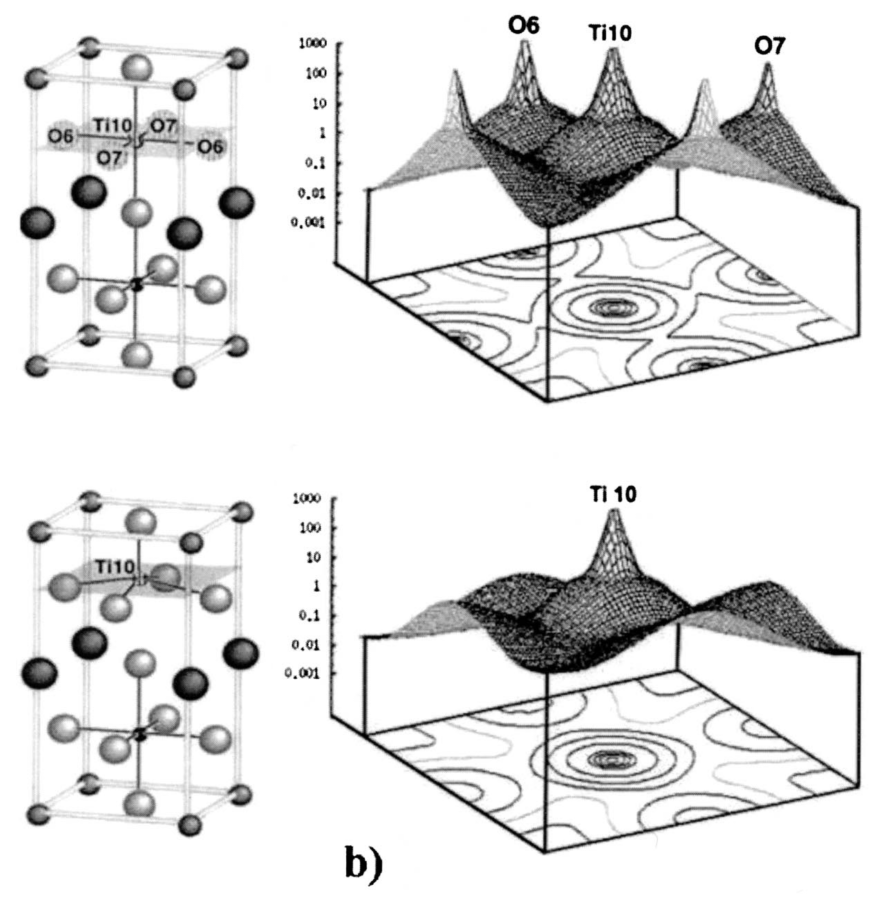
\includegraphics[width=0.95\textwidth]{longoB}
		\centering
	\end{minipage}
	\caption{Charge density from surface and contour plots from Longo et al. \cite{Longo2004} for crystalline and amorphous  Ba$_{0.5}$Sr$_{0.5}$TiO$_{3}$. (a) shows the vertical diagonal plane and (b) shows a horizontal plane.}
\end{figure}
\section{Molecular Dynamics}
\subsection{Formulation of Molecular Dynamics}
Molecular Dynamics (MD) is a classical method built off of

\begin{equation}
\vec{F}=m\vec{a} \qquad .
\end{equation}
Atoms are the smallest building block, represented as a sphere with a point mass \cite{Lee2012}. To calculate desired properties, atoms are allowed to ``relax" to their respective equilibrium distances, by moving down along the negative energy gradient:
\begin{equation}
\vec{F} = - \vec{\nabla} U \qquad .
\end{equation}
A calculation begins with a set of starting atomic coordinates. The energy is calculated and the atoms are adjusted, following the gradient, to a more stable position. The energy is again calculated and compared to the previous step. This process continues until the differences between subsequent energy values reaches a predetermined stopping value, e.g. a difference of 1 $\times 10^-4$ eV or less.
\par
This method requires selection of so-called pair-potentials, which describe how atom $i$ interacts with atom $j$. The simplest potential is the Lennard-Jones potential:

\begin{equation}
U_{ij}(r) = 4\epsilon \Bigg[\bigg(\frac{\sigma}{r}\bigg)^{12}-\bigg(\frac{\sigma}{r}\bigg)^{6}\Bigg] \qquad ,
\end{equation}
where $\epsilon$ is the depth of the energy well and $\sigma$ is the interatomic distance at which the potential is zero. However, this potential can only describe the interactions between atoms of the same element. In order to perform calculations on the majority of systems of interest, more complex pair-potentials are needed. Numerous potentials have been created, such as Embedded Atom Method (EAM) potentials which work for many metals and Tersoff potentials for covalent solids. 
\par 
An alternative method necessary for our discussion of AIMD in Section 5.1 is the Lagrangian:
\begin{equation}
L = K-U = \frac{1}{2}\sum_{i=1}^{3N}m_{i}v^{2}_{i}-U(r_{1}, \cdots, r_{3N})\qquad ,
\end{equation}
where $K$ is the kinetic energy, $U$ is the potential energy, and $N$ is the number of atoms.
\subsection{MD for the structure of alumina}
Guti\'errez et al. \cite{Gutierrez2002} used MD to investigate the structure of alumina. With the success of alloys and metals such as stainless steel, Ti, and Al largely attributed to their oxide layer, determining the structure of this oxide aids understanding of the passivation process. Guti\'errez used the pairwise potential
\begin{equation}
U(r_{ij})=\frac{q_{i}q_{j}}{r_{ij}}-\frac{C_{i}C_{j}}{r^{6}_{ij}}+D(B_{i}+B_{j})\exp\bigg(\frac{A_{i}+A_{j}-r_{ij}}{B_{i}+B){j}5}\bigg) \qquad ,
\end{equation}
where $r_{ij}$ is the interatomic distance between atoms $i$ and $j$, $D$ is the standard force constant 4.184 kJ/\AA$\cdot$mol., $q$ is the effective charge, $A$ is the repulsive radius, $B$ is the softness parameter, and $C$ is the van der Waals coefficient. This potential has been demonstrated to reproduce the structure, bulk modulus, thermal expansivities, melting temperatures, and liquid structure properties of Al$_{2}$O$_{3}$.
\begin{figure}[h]
	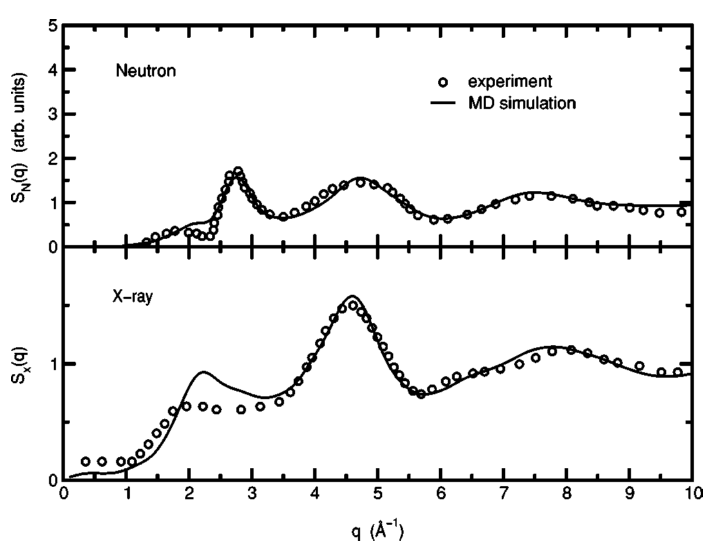
\includegraphics[width=0.6\textwidth]{gutierrez3}
	\centering
	\caption{MD results of Guti\'errez et al. \cite{Gutierrez2002} compared with experimental data for neutron and x-ray static structure function of Al$_{2}$O$_{3}.$} 
\end{figure}
\par
With a system of 1800 atoms, the researchers performed a melt-quench simulation by heating the system to 5000 K and evolving for 45 ps. Next the system was cooled to 3000 K at a rate of 1 K per 30 timesteps (1 fs). Finally, the system was allowed to equilibrate for 55 ps. Though these methods are known to be highly dependent on the melt-quench recipe, alternative initial configurations and quench rates were tested, but no discernible difference was found.
To perform statistical analysis of the structure, properties were averaged over 100 configurations: the last 100 structures, each 100 fs apart.

\begin{figure}[H]
	\centering
	\begin{minipage}[b]{0.45\textwidth}
		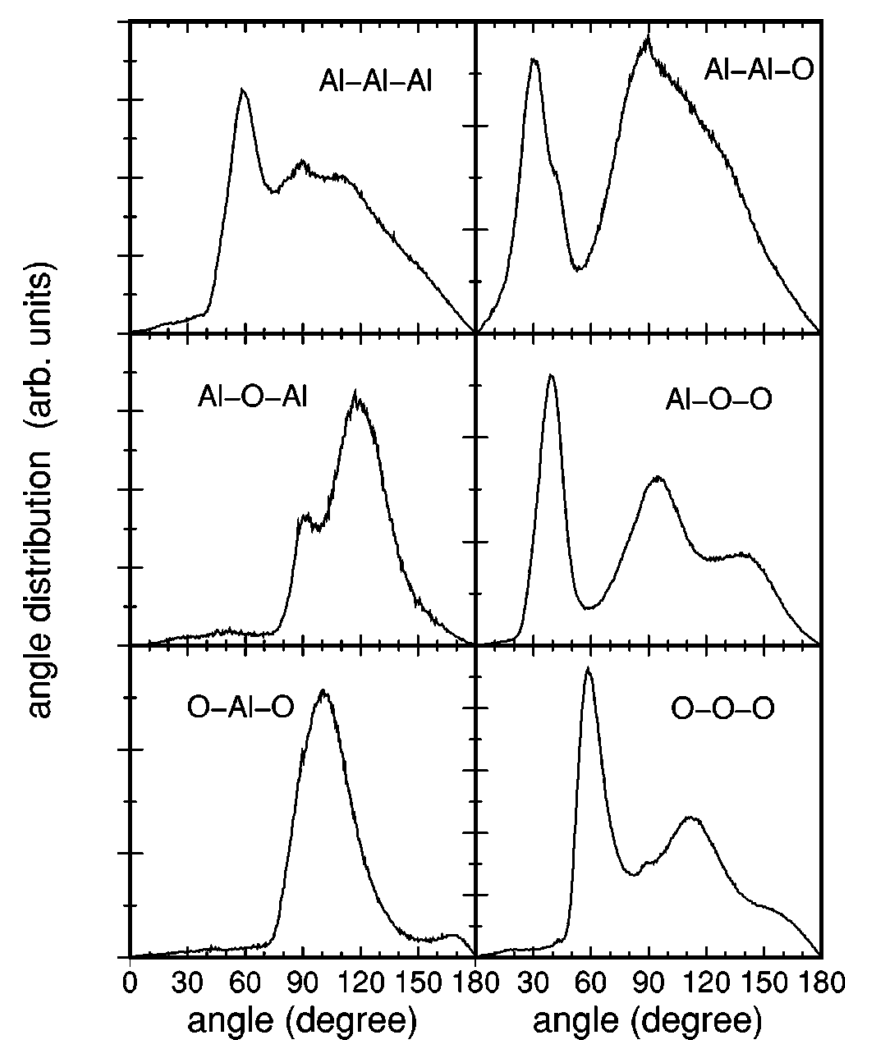
\includegraphics[width=0.94\textwidth]{gutierrez1}
		\caption{Results of Guti\'errez et al. \cite{Gutierrez2002} for bond angle distribution in amorphous Al$_{2}$O$_{3}$.}
	\end{minipage}
	\hfill
	\begin{minipage}[b]{0.45\textwidth}
		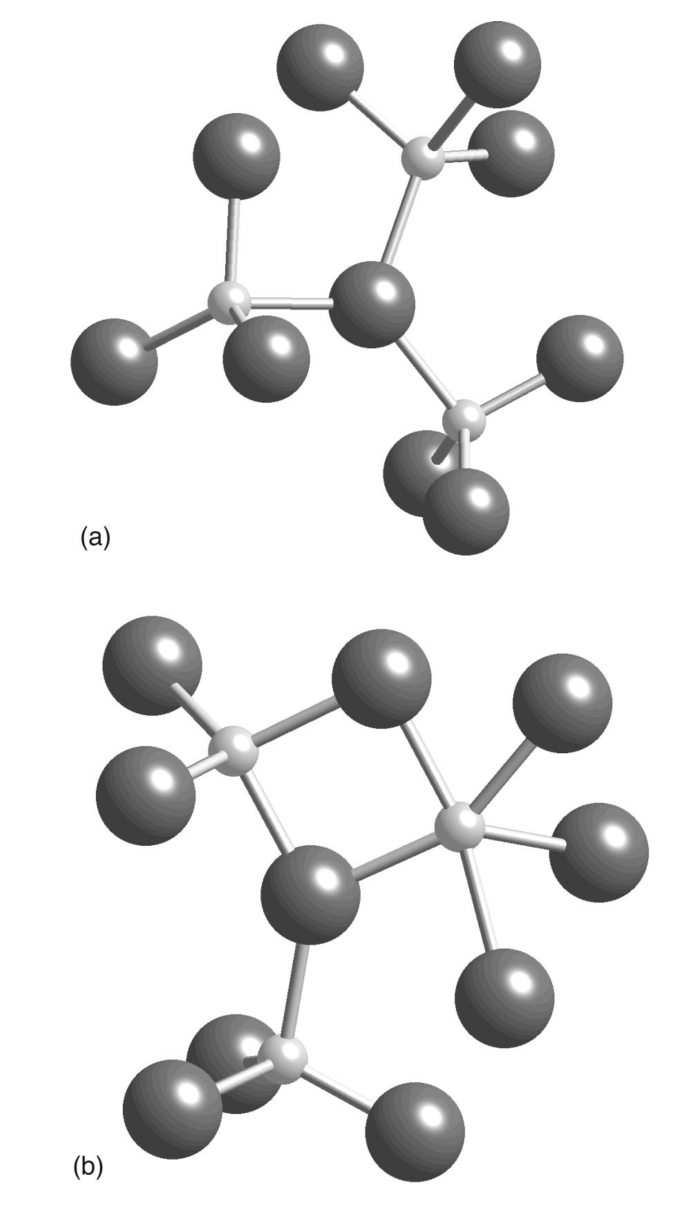
\includegraphics[width=0.55\textwidth]{gutierrez2}
		\centering
		\caption{Model suggested by Guti\'errez et al. \cite{Gutierrez2002} for basic Al$_{2}$O$_{3}$ units. (a) shows corner sharing tetrahedra while (b) shows edge-sharing polyhedra. Small and big spheres represent Al and O atoms, respectively. }
	\end{minipage}
\end{figure}
\par 
When compared with experimental structure factor, the results are in general agreement (\textbf{Fig. 7}). Though at low $q$ the results do not quite align, the simulation still shows a ``prepeak," consistent with experiment. From the bond-angle distribution shown in \textbf{Fig. 8}, the authors determined two structural motifs, as shown in \textbf{Fig. 9}.
%rings, gamma-alumina


\section{Monte Carlo}
Reverse Monte Carlo (RMC) algorithm can be used to find atomistic models from experimental data, commonly diffraction results. This large length scale method can produce unit cells on the order of thousands of atoms. The simulation begins with a unit cell with the desired atomic species and undergoes an iterative process of random atomic movements \cite{Cliffe2017}. If the movement creates a structure that better matches experiment, the movement is accepted. If the movement creates a structure yielding results less like diffraction data, the movement is rejected. Using this method in combination with DFT can help overcome the energetic barries to atomic reconfiguration. Cliffe et al. \cite{Cliffe2017} noted that creating stochastic models and relaxing with DFT can create unphysical structures. To avoid this problem, the authors used an RMC algorithm that is restrained to favor simpler solutions.
\par 
The authors began with a pair distribution function (PDF) generated from a  successful molecular dynamics model of a-Si referred to as WWW. Next, they created a random 512 atom unit cell and optimized the structure following

\begin{equation}
\chi = \frac{w_{PDF}}{N}\sum_{j}\sum_{r} \frac{[g_{j}(r)-g_{expt}(r)]}{r^{2}}+\frac{w_{L}}{N}\sum_{ij}L_{ij} \qquad ,
\end{equation}
where $N$ is the total number of atoms, $g_{j}(r)$ is the individual atomic radial distribution function, $g_{expt}$ is the experimental radial distribution function, $w_{PDF}$ is the weight of the PDF data, and $w_{L}$ is the weight of the self-similarity restraint. The self-similiarity is evaluated using the smooth overlap of atomic positions (SOAP) descriptor. This descriptor compares two atomic densities $\rho_{i}$ and $\rho_{j}$ over all rotations $\hat{R}$ and all positions $\vec{r}$:
\begin{equation}
k_{ij} = \int d \hat{R} \Bigg|\int d\vec{r}\rho_{i}(\vec{r})\rho_{j}(\vec{r})(\hat{R}\vec{r})\Bigg|^{2} \qquad .
\end{equation}
The authors also introduced an adaptive weighting scheme to confirm both self-similarity and PDF data contributed equally throughout the refinement. This was introduced as a scaling factor
\begin{equation}
A=\bigg(\frac{w_{PDF}\chi_{PDF}}{w_{L}\chi_{L}}\bigg)^{0.25} \qquad ,
\end{equation}
multiplied by the previous PDF weight and divided by the previous self-similarity rate. The results of this weighting scheme are shown in \textbf{Fig. 10}. 

\begin{figure}[H]
	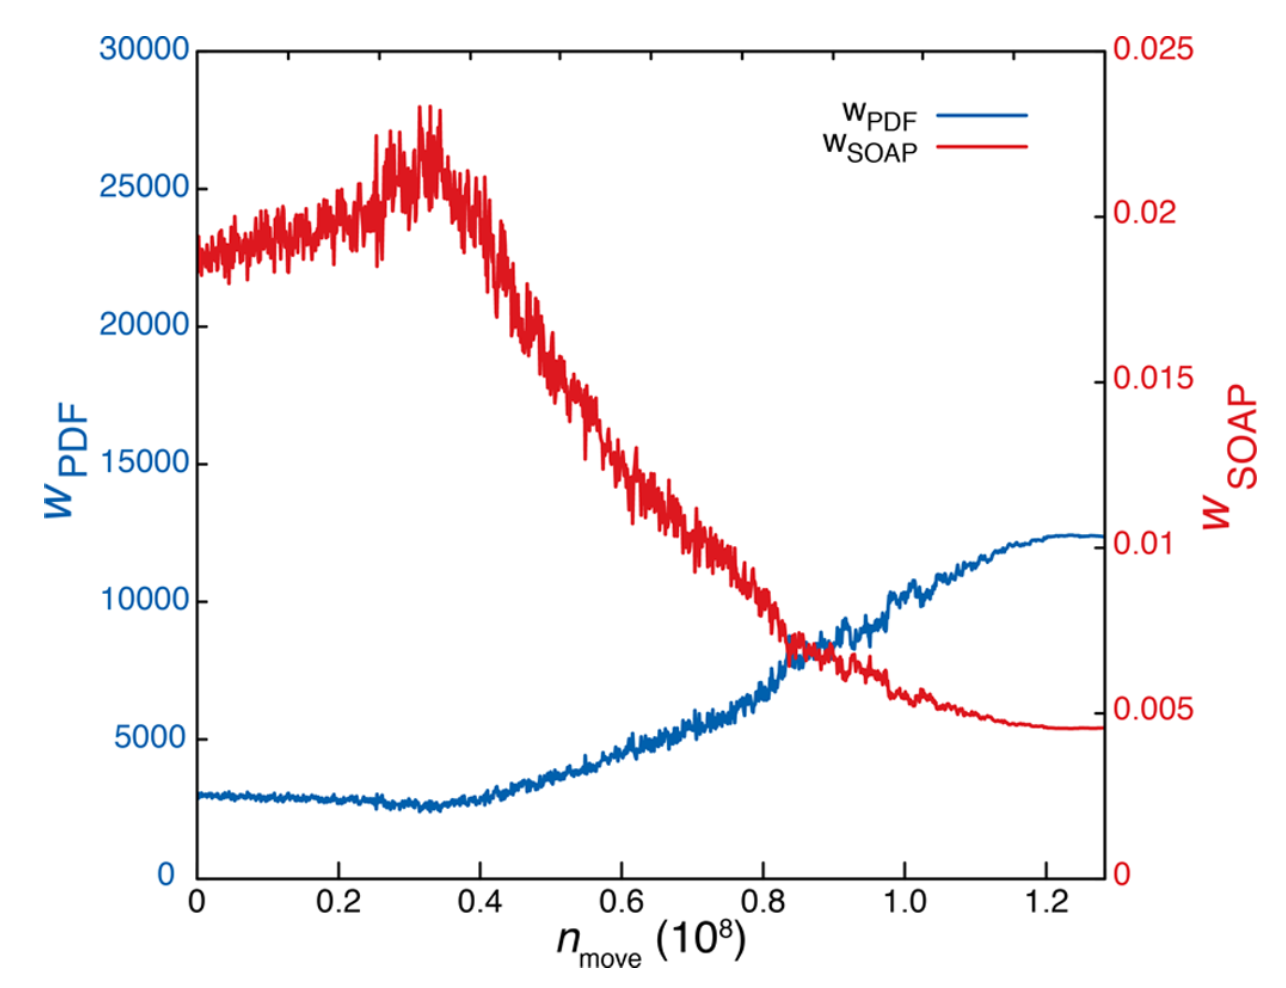
\includegraphics[width=0.35\textwidth]{white1}
	\centering
	\caption{Evolution of weighting scheme used by White et al. \cite{White2014}.}
\end{figure}

\begin{figure}[H]
	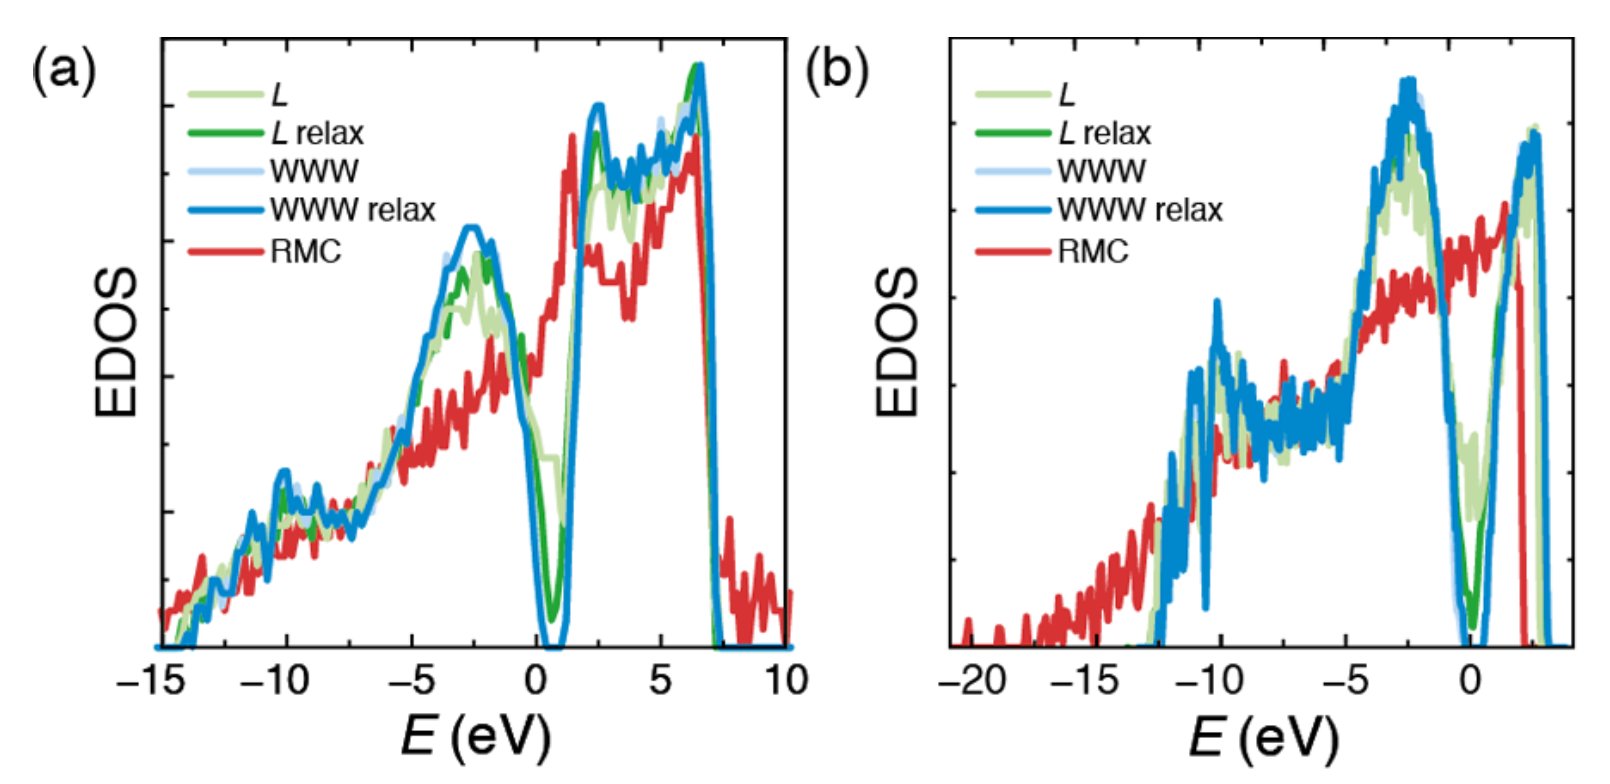
\includegraphics[width=0.6\textwidth]{white2}
	\centering
	\caption{Electronic density of states calculated from the (a) tight-binding model and the (b) MBJ meta-GGA functional for a-Si by Cliffe et al. \cite{Cliffe2017}. The density of states for unrestrained RMC is shown for comparison.}
\end{figure}

\par 
After obtaining the a-Si structure from L-constrained RMC, DFT calculations using the tight binding model were performed to obtain the electronic structure shown in \textbf{Fig. 11}. The unconstrained RMC DOS is rather featureless, while L-constrained RMC qualitatively reproduces the results of WWW. The authors double checked their results with the MBJ meta-GGA functional, known to accurately reproduce electronic properties of semiconductors, to confirm the results of their tight-binding model. Relaxation led to a slight deviation from the PDF data through the elimination of dangling-bond defects and, in turn, reduction in the density of gap states. Overall, this study demonstrates the utility in using simplity constraints on atomic relaxation.


















\section{\emph{Ab intio} Molecular Dynamics}
\subsection{Formulation of \emph{Ab initio} Molecular Dynamics}
\emph{Ab initio} Molecular Dynamics (AIMD) greatly extends the capabilities of both methods by advancing atoms along classical trajectories based on forces calculated from DFT\cite{Sholl2009}.
This is an incredibly powerful method that adds time treatment to DFT simulation while still allowing for \emph{ab initio} calculation of electronic properties. Furthermore, AIMD can circumvent the problem of metastable states, as shown for DFT+U \cite{Zhang2015}. This can be better conceptualized with the schematic of Car-Parrinello MD in \textbf{Fig. 12}. Instead of performing AIMD as a stepwise process in which calculating the atomic trajectories and the electronic ground state are separate, Car and Parinello formulated the two to run simultaneously. Their extended Lagrangian introduces the electronic degrees of freedom as fictitious dynamical variables:
\begin{equation}
L =\frac{1}{2}\sum_{i=1}^{3N}m_{i}v^{2}_{i}-U(r_{1}, \cdots, r_{3N})+\frac{1}{2}\sum_{j}2\mu \int d\vec{r}|\dot{\psi}(\vec{r})|^{2}+L_{ortho}
\end{equation}
The third term introduces fictitious mass, $\mu$, and the final term restrains the one-electron wave functions to be orthogonal. Since the total energy calculation occurs simultaneously with the atomic trajectory calculation, the energy is not quite the same as the energy calculated with pure DFT, as shown in \textbf{Fig. 12}. This phenemona circumvents the structure getting trapped in a metastable state, as DFT methods are known to do \cite{Dorado2013}.
\begin{figure}[h]
	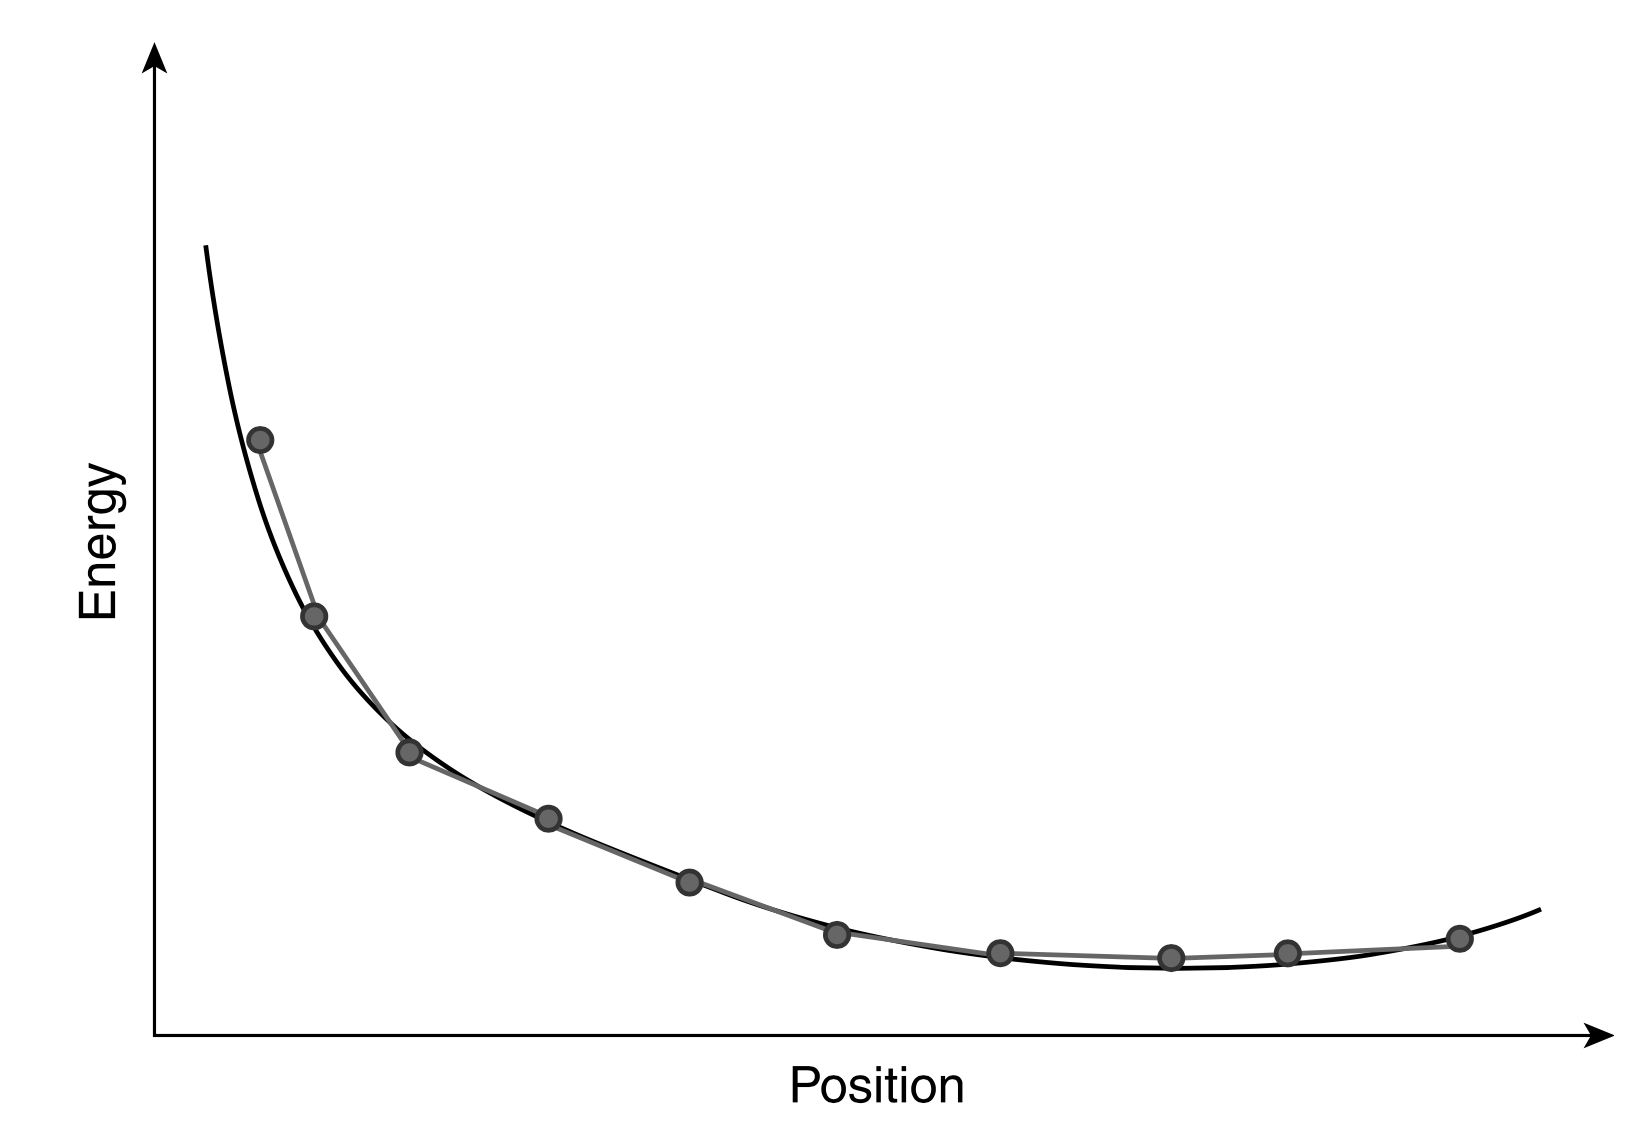
\includegraphics[width=0.5\textwidth]{practical1}
	\centering
	\caption{Schematic of Car-Parrinello MD trajectory along a single coordinate \cite{Sholl2009}. The smooth curve gives the exact electronic ground state energy, while the circles show the electronic energy calculated by Car-Parrinello MD at each step of the MD simulation.} 
\end{figure}

\par
Shortly after the formulation of Car-Parrinello MD, Car and Parrinello realized the utility of the method for amorphous materials \cite{Car1988}. They discussed the dependence of MD and MC on interatomic potentials. As potentials are fitted to experimental data, the validity of the model in other applications cannot be assessed. Furthermore, it is difficult to determine the electronic properties and atomic dynamics that give rise todevice performance. In contrast, AIMD allows for calculation of the potential directly from first principles.

\subsection{AIMD for Phase Change Memory}
Raty et al. \cite{Raty2015} used Ab Initio Molecular Dynamics to understand the structural changes associated with aging in GeTe, and the effects those changes have on performance. Inherently out of equilibrium, amorphous materials evolve with time to a lower energetic state. In the case of phase change materials, this evolution leads to higher electrical resistivity that undermines its usability in multilevel memory devices. Using AIMD, we can watch the structure evolve, but though AIMD adds time to DFT, this time is still on the order of picoseconds, leaving real-time aging out of the question. Raty et al. have side-stepped this problem by creating an arrangement of structures with varying local motifs. 
\par
Their study begins with the observation that AIMD simulations of Ge$_{x}$Sb$_{y}$Te$_{1+x+y}$ alloys show tetrahedrally bonded Ge (Ge$^{T}$) atoms in the amorphous phase, though these are absent in crystalline Ge. To investigate the effect of such homopolar bonds on GeTe properties, the authors melt-quenched GeTe along with a combination of other binary chalcogenides for use as``templates." SiTe forms numerous Si$^{T}$, GeSe contains some Ge$^{T}$, and SnTe contains almost no tetrahedral motifs.  The authors then substituted one species in each of the template compounds to form GeTe, i.e. substituting Si in SiTe with Ge, Se in GeSe with Te, and Sn in SnTe with Ge. After substitution, the systems were subjected to a shorter additional melt-quench procedure.
\begin{figure}[h]
	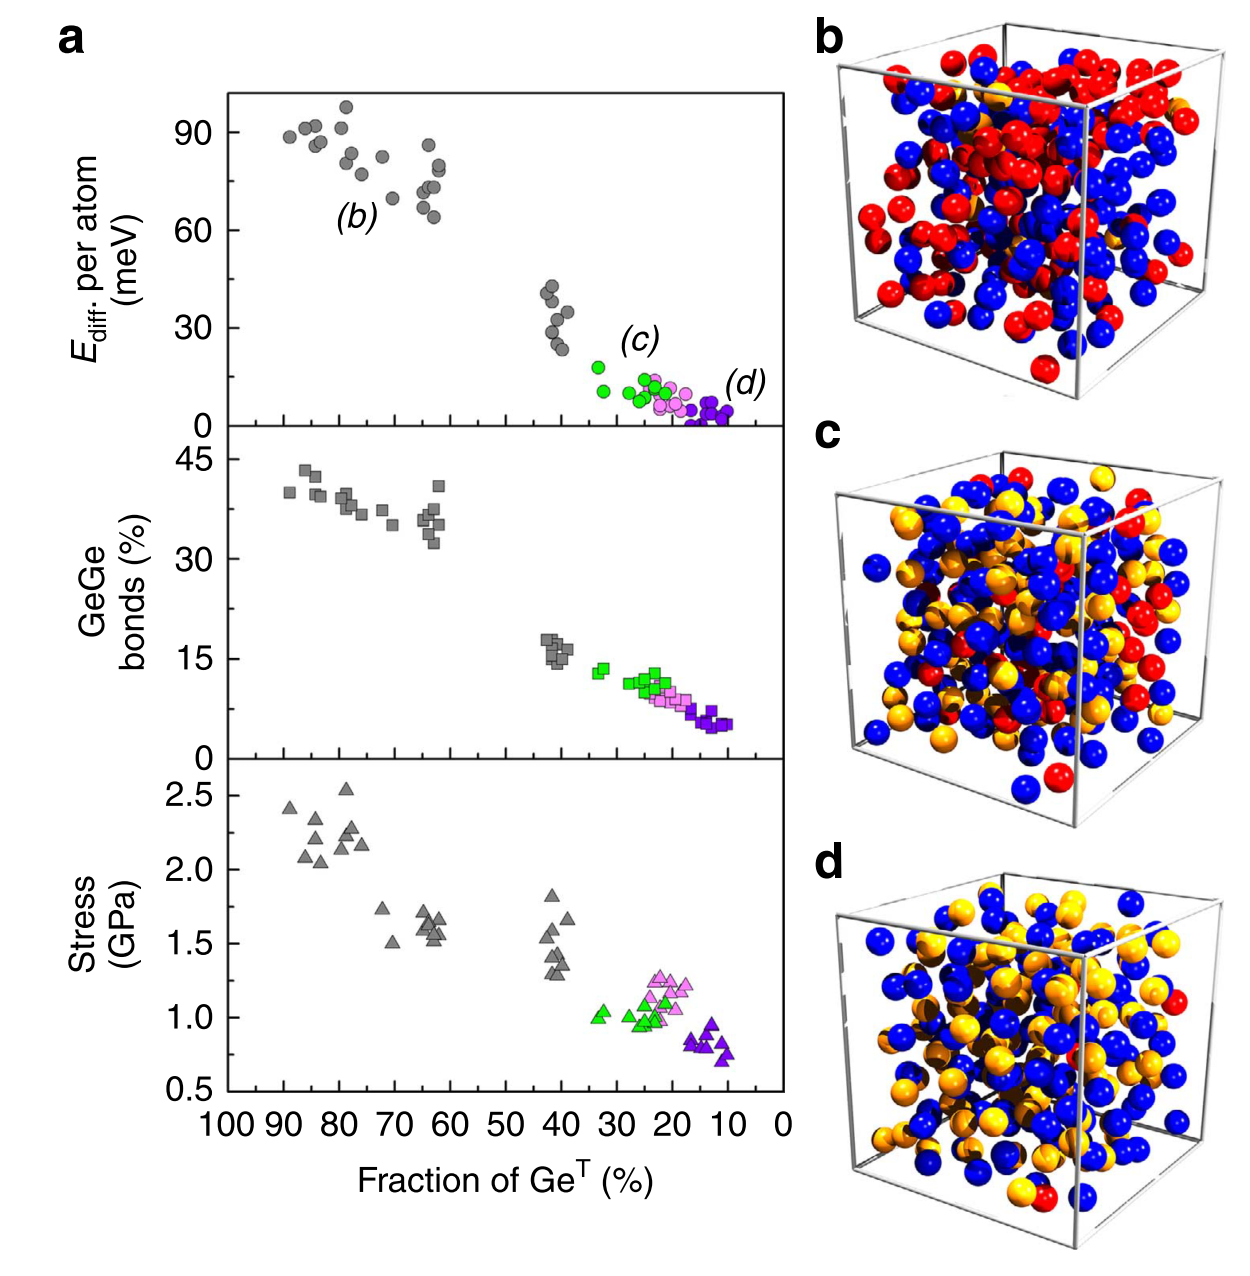
\includegraphics[width=0.5\textwidth]{raty1}
	\centering
	\caption{Results from Raty et al. \cite{Raty2015} for (a) the energy difference per atom, fraction of homopolar GeGe bonds, and stress of the melt-quenching of GeTe (green) and chemical replacement systems SnTe (violet), GeSe (pink), and SiTe (grey). (b-d) show the atomic configurations of GeTe as labeled in the energy difference plot. Te, tetrahedral Ge, and octahedral Ge are rendered in blue, red, and orange, respectively.} 
\end{figure}
\par 
The results shown in \textbf{Fig. 13(a)} indicate that the homopolar bonds reduce the stability of the system. However, homopolar bonds have a lower heat of formation in GeTe than in both GeSe and SnTe, and the melt-quench process is able to stabilize these tetrahedral motifs. In comparison to experiment, aging of phase change materials has been linked with stress relief. These results suggest that the removal of homopolar bonds contributes to this stress relief.
\par 
Raty et al. additionally calculated the changes in the electronic and optical bandgaps due to the changes in percent Ge$^{T}$. Though methods of calculating optical properties are beyond the scope of this review, the results of Raty et al. for the optical bandgap in \textbf{Fig. 14(a)} and \textbf{Fig. 15} show increasing band gap correlated with decreasing homopolar bonds, in agreement with experiment showing band gap widening with aging. Similarly, the DOS shows an increase in electronic band gap with aging, and the disappearance of the midgap states are directly linked to the removal of homopolar bonds. The authors note that while a variety of Ge$^T$ concentrations have been modeled, this method does not yield access to the time scale of the relaxation process. 
\begin{figure}[H]
	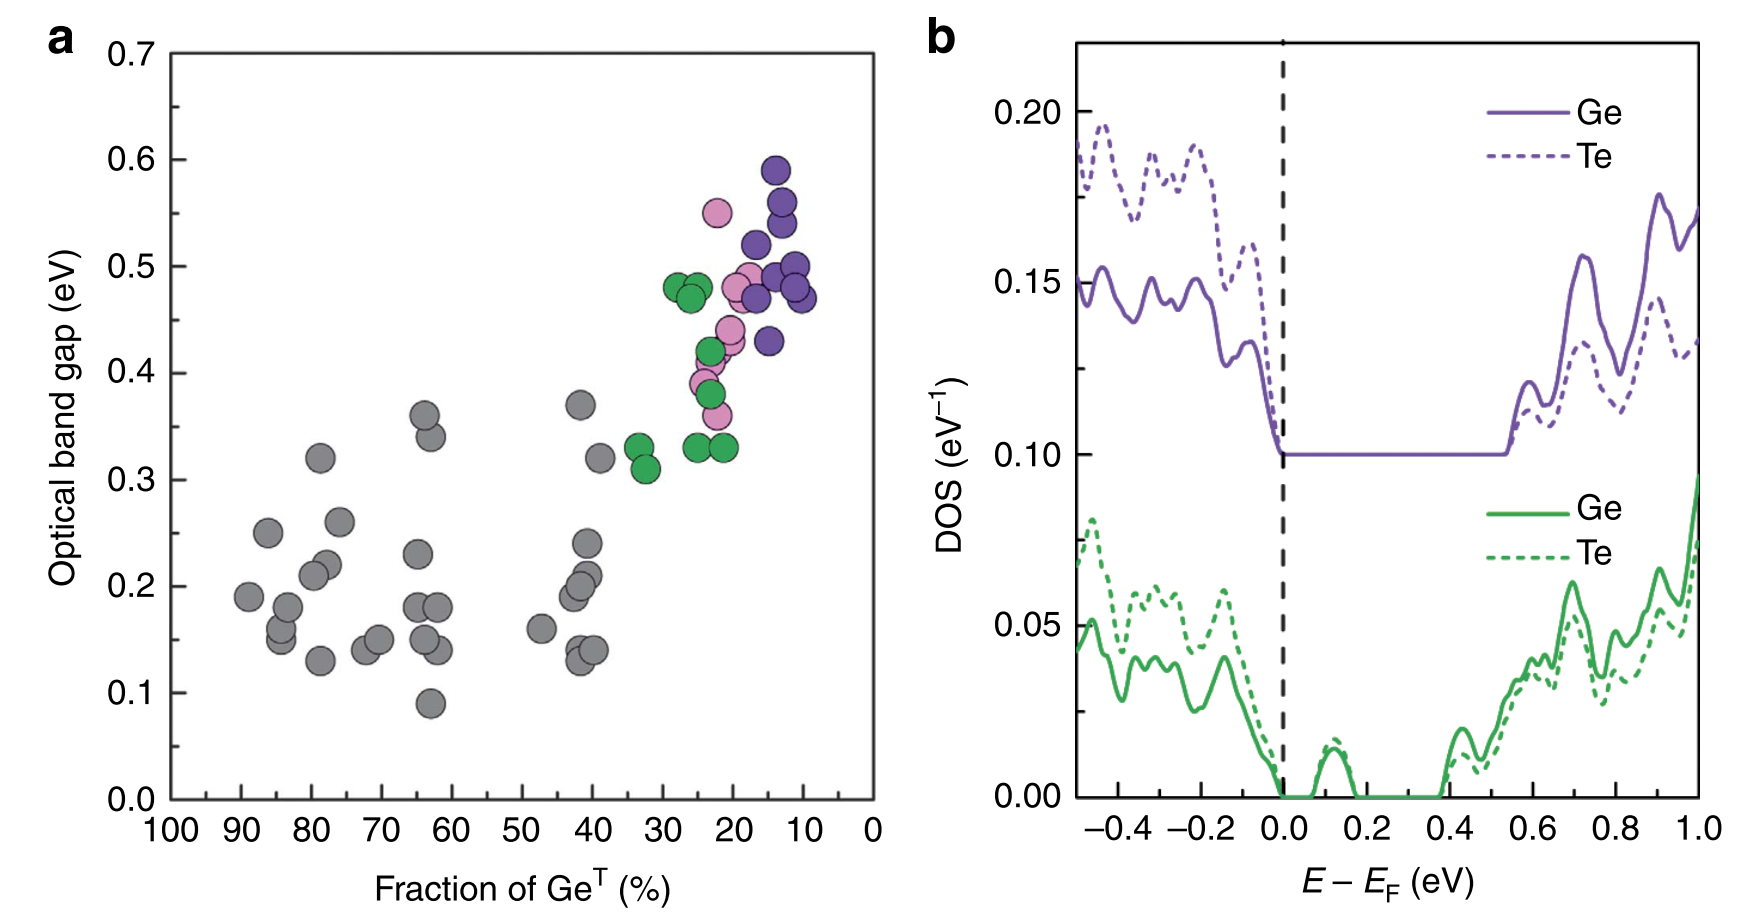
\includegraphics[width=0.5\textwidth]{raty2}
	\centering
	\caption{Results from Raty et al. \cite{Raty2015} for (a) the relaxed amorphous GeTe structures as a function of percent Ge$^{T}$ and (b) the local density of states for melt-quenched GeTe (green) and substituted a-SnTe (violet).}
\end{figure}

\begin{figure}[H]
	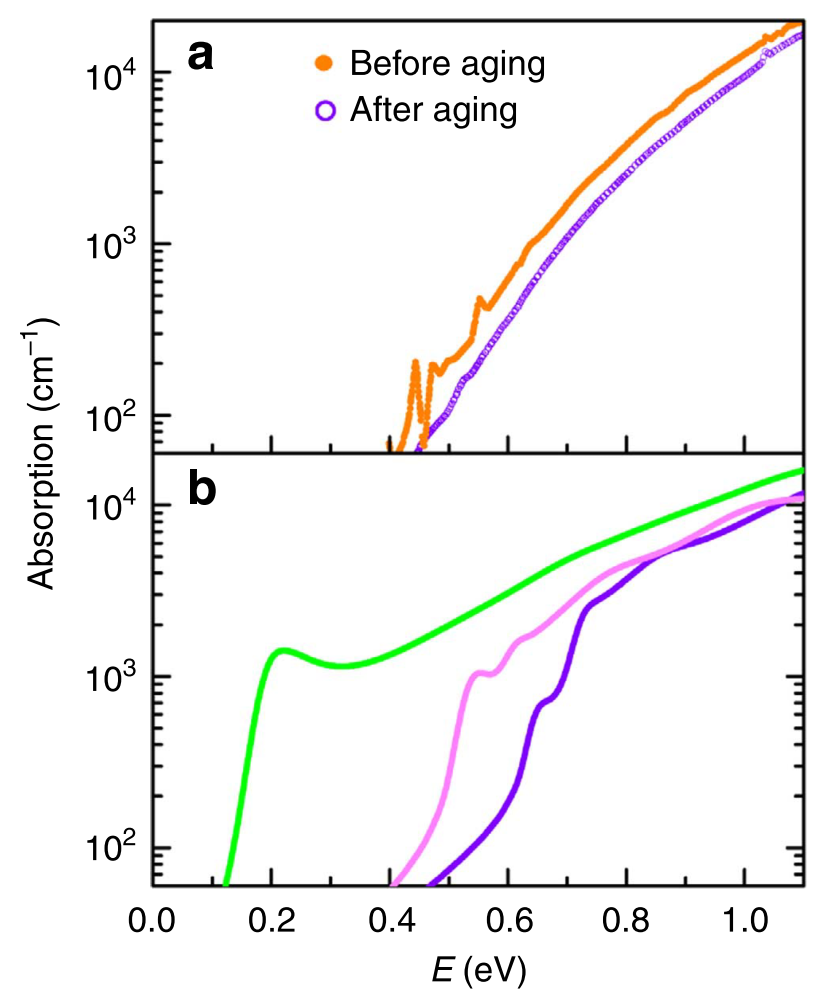
\includegraphics[width=0.3\textwidth]{raty3}
	\centering
	\caption{Results from Raty et al. \cite{Raty2015} for (a) experimental absorption from photothermal deflection spectroscopy (PDS) and (b) calculated absorption oscillator strength for melt-quenched GeTe (green), substituted a-GeSe (pink), and substituted a-Sn-Te (violet). } 
\end{figure}






\section{Discussion}
DFT allows for the calculation of total energy, band structure, density of states, bulk modulus, magnetic moment, among other properties. While the method can be highly accurate, it sometimes runs into the issue of reaching metastable states \cite{Dorado2013}. If the achieved structure is not the true ground state, it may inaccurately represent the structure and the properties calculated from it. Additionally, due to computational expense DFT can only be reasonable performed for systems of less than 100 atoms.
\par 
MD can treat hundreds of atoms, as well as include the effects of time, temperature, and pressure. This is allows for studies including the temporal evolution of a system and heat treatment. However, it relies on the selection of a pair-potential. Even state-of-the-art pair-potentials can struggle to describe anisotropic systems \cite{Hohl1991}. Additionally, due to their empirical nature, a potential may not always describe properties other than those it was designed for \cite{Cliffe2017, Car1988}. For instance, if an interatomic potential is fitted to structural properties, it will not necessarily reproduce magnetic properties. Furthermore, it may not be able to treat new materials that have not been studied experimentally.
\par 
MC can treat thousands of atoms, but like Molecular Dynamics is hindered by the need for interatomic potentials \cite{Car1988}. Reverse Monte Carlo, on the other hand, can identify thousands of atom unit cells from experimental data. Again, this requires previously conducted experiments and thus cannot be used for screening.
\par 
AIMD circumvents the empirical interatomic potential problem by calculating potentials on-the-fly with DFT.  This both adds the time dimension to DFT and allows for the calculation of electronic properties from MD. Still, it cannot feasibly model as many atoms and as large time scales as MD and above.
\par 
Selecting a method requires a clear definition of the system and project goals. To determine electronic properties, one should use DFT or AIMD. To determine large scale properties or even temporal evolution, one should use MD or MC. Consider how large of a unit cell is needed for the study, what time scale should it run on, and what takes priority: time of study or accuracy? Is the goal to screen for the optimal material or to understand an observed property? In the case of DFT and AIMD, carefully select your exchange-correlation functional. If your priority is getting results quickly, GGA will likely suffice. If your priority is a very accurate calculation, try a hybrid functional and verify in the literature that this functional can describe your system or systems like it. In the case of MD and MC, select a pair-potential that is accurate for your system and balance your needs of speed of calculation vs. accuracy. Regardless of method, a strong understanding of the formulation will aid the researcher in identifying in what cases the method fails and in what cases the method can answer desired questions.




\section{Conclusions}
We have examined four computational methods applicable to amorphous materials: DFT, AIMD, MD, and MC. DFT has been used to identify the structure leading to photoluminescence in amorphous perovskites \cite{Longo2004}. As Ti shifts to create five- and six-fold coordination, this creates localized states on the O that subsequently reduce the band gap. Electronic structure results show the indirect and direct band gap values and the density of states for each atom. Partial charge density was used to visualize the electronic structure and identify ionic and covalent bonding. 
MD has been used to determine the statistical bond angles present in amorphous alumina, providing insight on the structural motifs present \cite{Gutierrez2002}. Reverse Monte Carlo was used to show the positive results from preferring simplicity and the additional details this can lead to in the electronic properties \cite{Cliffe2017}. AIMD has been used to find the relation between homopolar bonds and aging, altering both electronic and optical properties \cite{Raty2015}.
\par Though no one method can describe all length and time scales, each as strengths in different areas. When selecting a method for study, one should carefully consider their system and the needs of their study. Once a method is chosen appropriately, it can be used to find structures and mechanisms unattainable through experiment. Also, while such examples were not discussed here, computational methods can  be used to screen prospective materials to predict which will yield the best properties. Multiscale modeling, or coupling of methods across length scales, has gained increasing attention for holistically describing materials \cite{DePablo2007}. Such an endeavor may one day benefit amorphous materials. Ultimately, by using computation, amorphous materials can be better understood.




\section*{References}

\bibliography{amorph}
\bibliographystyle{elsarticle-num}

\end{document}  